\documentclass{article}
\usepackage{multicol}
\usepackage{graphicx}
\usepackage{xcolor}
\definecolor{keyword}{rgb}{0.3568627451, 0.7372549020, 0.6431372549}
\definecolor{comment}{rgb}{0.5411764706, 0.7490196078, 0.3450980392}
\definecolor{string}{rgb}{0.9,0.4,0}
\definecolor{function}{rgb}{0.5,0.5,0.1}
\usepackage{listings}
\lstset{
    basicstyle=\small\ttfamily,
    breaklines=true,
    frame=single,
    rulecolor = \color{gray},
    numbers=left,
    numbersep=5pt,
    numberstyle=\tiny,
    showstringspaces=false,
    tabsize=4,
    keywordstyle=\color{keyword},
    commentstyle=\color{comment},
    stringstyle=\color{string},
}
\usepackage{hyperref}
\hypersetup{
    colorlinks=true,
    urlcolor=cyan,
}
\usepackage{makecell}
\usepackage[a4paper, margin=1in]{geometry}
\usepackage{float}

\title{Cloud Computing - Project Report \\ \small{Totoro Group}}
\author{
    Zahra Omrani \\ z.omrani@studenti.unipi.it \and 
    Paolo Palumbo \\ p.palumbo3@studenti.unipi.it \and
    Ettore Ricci \\ e.ricci32@studenti.unipi.it}

\begin{document}
\maketitle
\begin{center}
    \scriptsize
    \href{https://github.com/Etto48/CloudComputingProject}{https://github.com/Etto48/CloudComputingProject}
\end{center}

\begin{abstract}
    This report presents the development and performance evaluation of a Java-based application 
    designed to count letter frequencies in large datasets using the Hadoop framework. 
    To provide a comprehensive analysis, we also implemented and tested non-distributed 
    applications in Python and Rust for comparison.
    The results show that for the sizes of the datasets considered, Java and Python execution 
    times are comparable, while Rust is significantly faster. 
    Both Python and Rust applications used significantly less memory than the Java application.
\end{abstract}
\begin{multicols}{2}
\section{Introduction}
    Our project for the Cloud Computing course consists of developing a Java application to count
    the frequency of letters in a large dataset using the Hadoop framework.
    The main objective of the project is to analyze and compare the performance of the application
    with different configurations and input sizes and also to compare it with non-distributed
    implementations in Python and Rust.
\section{Mapreduce}
    MapReduce is a programming model for processing large data sets. 
    Users specify a map function that processes a key/value pair to generate a set
    of intermediate key/value pairs, and a reduce function that merges all intermediate values
    associated with the same intermediate key.
\subsection{Mapper}
    The Mapper class is responsible for processing the input data and generating a set of key/value pairs.
    In our case the input data is a piece of text, the key is a letter and the value is the number of 
    occurrencies of that letter.
    To count the occurrencies of each letter we first transformed the input text to ascii (normalizing accented
    letters) and then we counted the occurrencies of each letter.
    For this project we tested two different mappers:
    \begin{itemize}
        \item \textbf{In-mapper combiner}: (Listing \ref{lst:java_mapper}) 
        For the in-mapper combiner, we used a vector of size 26 to store the frequency of each letter and
        another variable to store the total number of letters. During the map phase, we update the vector
        and the total count for each letter. In the cleanup phase, we emith for each letter its occurrencies 
        and the total count.
        \item \textbf{No in-mapper combiner}: (Listing \ref{lst:java_mapper_no_combiner})
        For the mapper without in-mapper combiner, we emit a key-value pair for each letter in the input text
        containing the letter and the number 1.
    \end{itemize}
    The key is a custom class called Char (Listing \ref{lst:java_char}) and the value is a custom class 
    called CountTotalPairWritable (Listing \ref{lst:java_count_total_pair}).
    We used custom classes to optimize the memory usage and the serialization/deserialization process.
\subsection{Reducer}
    (Listing \ref{lst:java_reducer}) 
    The Reducer class is responsible for processing the intermediate key/value pairs generated by the Mapper
    and generating the final output. In our case, the reducer receives a letter and a list of pairs of 
    its occurrencies and total letters count. The reducer sums the occurrencies of each letter and then 
    calculates the frequency of each letter.
\section{Dataset}
    We used three different datasets:
    \begin{itemize}
        \item \textbf{english.txt}: A 1.2GB text file containing text from the books on Gutenberg project.
        \item \textbf{italian.txt}: A 1.3GB text file from the PAISÀ corpus.
        \item \textbf{spanish.txt}: A 130MB text file from the Leipzig Corpora Collection.
    \end{itemize}
    We also created 11 files of increasing size (from 100MB to 1.1GB with 100MB steps) to test the performance
    of the application with different input sizes. These files are called \textbf{part\_$X$MB.txt} and 
    contain the first $X$MBs of the \textbf{english.txt} file. 
\section{Experiments}
\section{Results}
\begin{figure}[H]
    \centering
    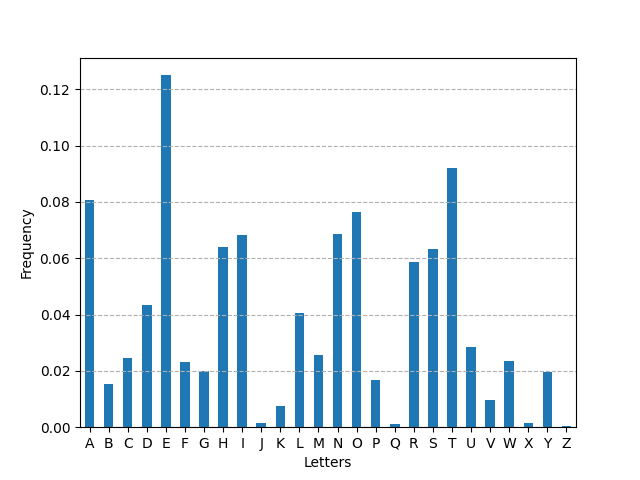
\includegraphics[width=0.48\textwidth]{figures/en.png}
    \caption{English letter frequency}
    \label{fig:en_freq}
\end{figure}
\begin{figure}[H]
    \centering
    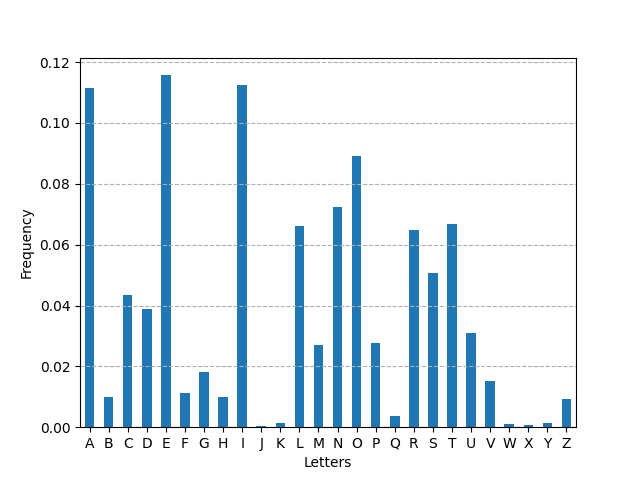
\includegraphics[width=0.48\textwidth]{figures/it.png}
    \caption{Italian letter frequency}
    \label{fig:it_freq}
\end{figure}
\begin{figure}[H]
    \centering
    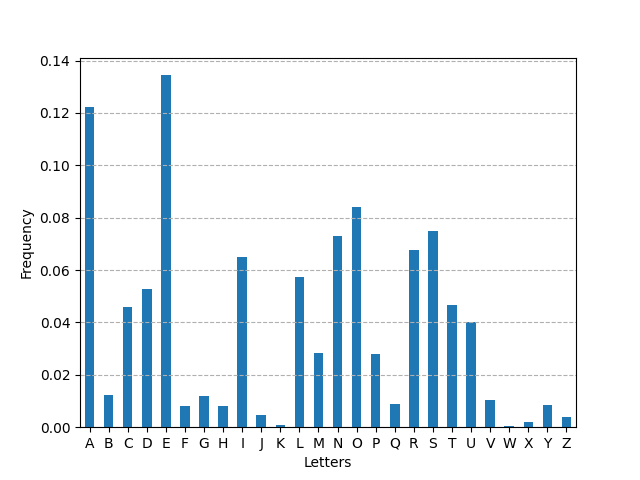
\includegraphics[width=0.48\textwidth]{figures/es.png}
    \caption{Spanish letter frequency}
    \label{fig:es_freq}
\end{figure}

\begin{table}[H]
    \centering
    \begin{tabular}{|c|l|}
        \hline
        Test ID & Arguments \\
        \hline
        0 & \makecell[l]{-i english.txt \\ -r 1} \\        
        \hline
        1 & \makecell[l]{-i english.txt \\ -r 2} \\        
        \hline
        2 & \makecell[l]{-i english.txt \\ -r 4} \\        
        \hline
        3 & \makecell[l]{-i english.txt \\ -r 8} \\        
        \hline
        4 & \makecell[l]{-i english.txt \\ -r 1 \\ --no-combiner} \\        
        \hline
        5 & \makecell[l]{-i english.txt \\ -r 1 \\ --no-in-mapper-combiner} \\        
        \hline
        6 & \makecell[l]{-i english.txt \\ -r 1 \\ --no-in-mapper-combiner \\ --no-combiner} \\        
        \hline
        7 & \makecell[l]{-i english.txt \\ -r 4 \\ --no-combiner} \\        
        \hline
        8 & \makecell[l]{-i english.txt \\ -r 4 \\ --no-in-mapper-combiner} \\        
        \hline
        9 & \makecell[l]{-i english.txt \\ -r 4 \\ --no-in-mapper-combiner \\ --no-combiner} \\        
        \hline
    \end{tabular}
    \caption{General tests}
    \label{tab:general_tests}
\end{table}
\begin{table}[H]
    \centering
    \begin{tabular}{|c|l|}
        \hline
        Test ID & Arguments \\
        \hline
        10 & \makecell[l]{-i part\_100MB.txt \\ -r 1} \\  
        \hline      
        11 & \makecell[l]{-i part\_200MB.txt \\ -r 1} \\  
        \hline      
        12 & \makecell[l]{-i part\_300MB.txt \\ -r 1} \\        
        \hline
        13 & \makecell[l]{-i part\_400MB.txt \\ -r 1} \\        
        \hline
        14 & \makecell[l]{-i part\_500MB.txt \\ -r 1} \\        
        \hline
        15 & \makecell[l]{-i part\_600MB.txt \\ -r 1} \\        
        \hline
        16 & \makecell[l]{-i part\_700MB.txt \\ -r 1} \\        
        \hline
        17 & \makecell[l]{-i part\_800MB.txt \\ -r 1} \\        
        \hline
        18 & \makecell[l]{-i part\_900MB.txt \\ -r 1} \\        
        \hline
        19 & \makecell[l]{-i part\_1000MB.txt \\ -r 1} \\        
        \hline
        20 & \makecell[l]{-i part\_1100MB.txt \\ -r 1} \\            
        \hline
    \end{tabular}
    \caption{Input split tests}
    \label{tab:input_split_tests}
\end{table}

\end{multicols}
\begin{figure}[H]
    \centering
    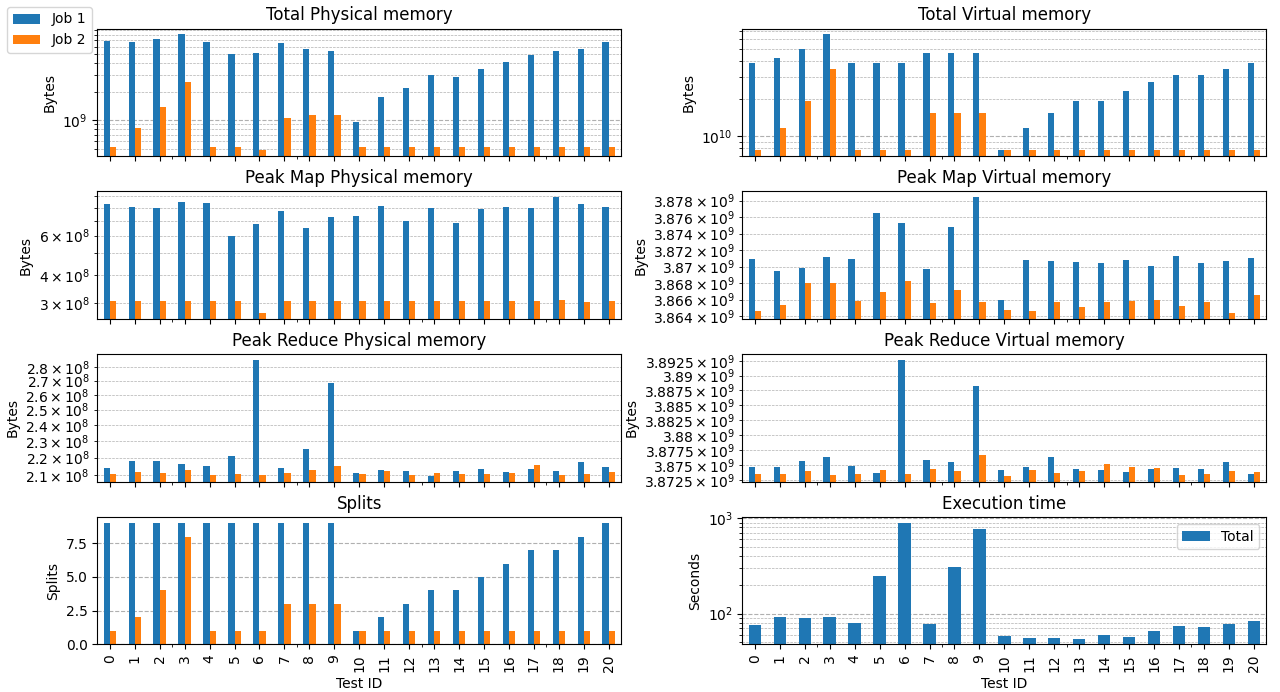
\includegraphics[width=1\textwidth]{figures/experiments.png}
    \caption{Tests results, the x-axis represents the test ID.}
    \label{fig:tests_graph}
\end{figure}
\begin{multicols}{2}
\begin{figure}[H]
    \centering
    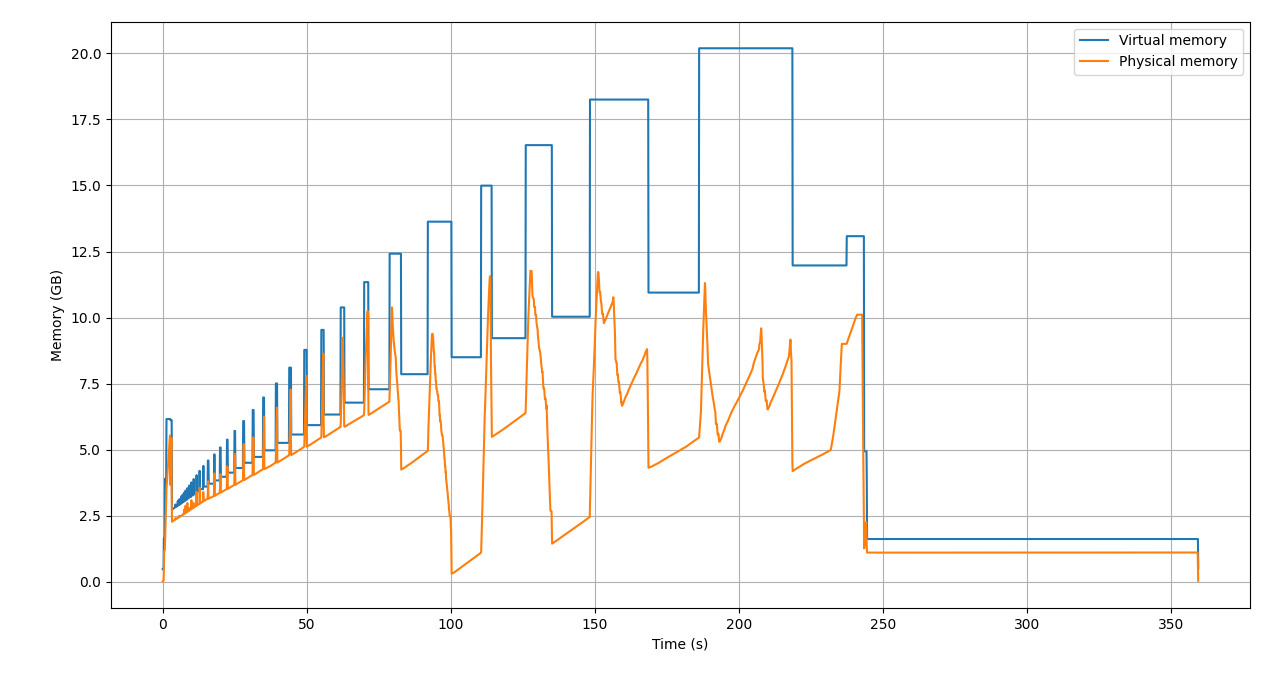
\includegraphics[width=0.48\textwidth]{figures/baseline_py.png}
    \caption{Python baseline memory usage (GB) over time (s)}
    \label{fig:baseline_py}
\end{figure}
\begin{figure}[H]
    \centering
    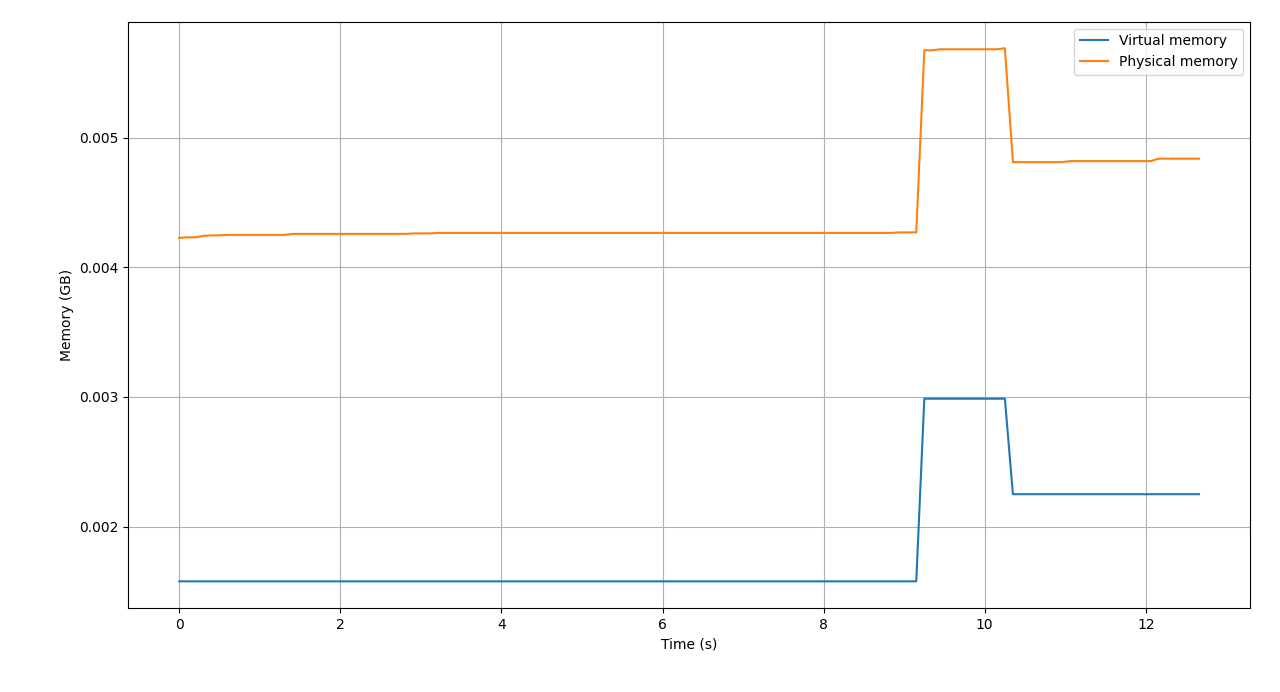
\includegraphics[width=0.48\textwidth]{figures/baseline_rs.png}
    \caption{Rust baseline memory usage (GB) over time (s)}
    \label{fig:baseline_rs}
\end{figure}

\section{Conclusions}
\end{multicols}
\section{Listings}
\lstinputlisting[
    language=Java, 
    caption={Mapper with in-mapper combiner},
    label={lst:java_mapper}
]{../letterfreq/src/main/java/it/unipi/Mapper.java}
\lstinputlisting[
    language=Java,
    caption={Mapper without in-mapper combiner},
    label={lst:java_mapper_no_combiner}
]{../letterfreq/src/main/java/it/unipi/MapperNoCombiner.java}
\lstinputlisting[
    language=Java,
    caption={Reducer},
    label={lst:java_reducer}
]{../letterfreq/src/main/java/it/unipi/Reducer.java}
\lstinputlisting[
    language=Java,
    caption={ReducerFrequency class, used to calculate the frequency of each letter},
    label={lst:java_reducer_frequency}
]{../letterfreq/src/main/java/it/unipi/ReducerFrequency.java}
\lstinputlisting[
    language=Java,
    caption={Char class, used as a custom key},
    label={lst:java_char}
]{../letterfreq/src/main/java/it/unipi/Char.java}

\end{document}